\documentclass{article}
\usepackage{thumbpdf}
\usepackage[pdftex,
        colorlinks=true,
        urlcolor=rltblue,       % \href{...}{...} external (URL)
        filecolor=rltgreen,     % \href{...} local file
        linkcolor=rltred,       % \ref{...} and \pageref{...}
        pdftitle={Untitled},
        pdfauthor={Your Name},
        pdfsubject={Just a test},
        pdfkeywords={test, testing, testable stuff},
        pdfproducer={pdfLaTeX},
        pagebackref,
        pdfpagemode=UseNone,
        bookmarksopen=true]{hyperref}
\usepackage{color}
\definecolor{rltred}{rgb}{0.75,0,0}
\definecolor{rltgreen}{rgb}{0,0.5,0}
\definecolor{rltblue}{rgb}{0,0,0.75}
\usepackage{tikz}

\title{Untitled}
\author{Your Name}
\date{\today}

\begin{document}\label{start}

\maketitle

\section{Section One}

A test document from
\href{http://www.Ringlord.com/}{Ringlord Technologies}!

\subsection{Subsection One Dot One}

Hello, this is section 1.1

\subsection{Subsection One Dot Two}

And here we have section 1.2; here's a link to
\href{Other.pdf}{another Document (Other.pdf)},
which probably does not exist (but that's OK).

\section{Section Two}

You could also click on the following number to jump to
the first page, namely page \pageref{start}\ldots

% Sketch output, version 0.3 (build 7d, Wed May 2 06:36:52 2012)
% Output language: PGF/TikZ,LaTeX
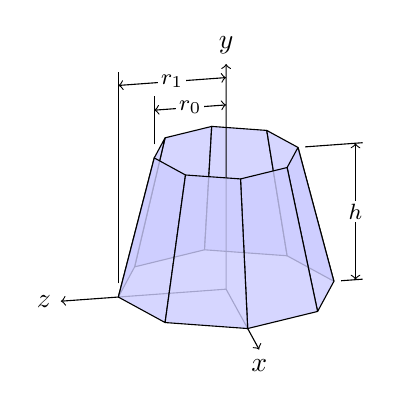
\begin{tikzpicture}[line join=round]
\tikzstyle{ann} = [fill=white,font=\footnotesize,inner sep=1pt]\filldraw[fill=blue!20,fill opacity=0.8](-.775,1.922)--(-1.162,.283)--(-.274,.5)--(-.183,2.067)--cycle;
\filldraw[fill=blue!20,fill opacity=0.8](-.183,2.067)--(-.274,.5)--(.775,.424)--(.516,2.016)--cycle;
\filldraw[fill=blue!20,fill opacity=0.8](.516,2.016)--(.775,.424)--(1.369,.1)--(.913,1.8)--cycle;
\filldraw[fill=blue!20,fill opacity=0.8](-.913,1.667)--(-1.369,-.1)--(-1.162,.283)--(-.775,1.922)--cycle;
\draw(1.461,.107)--(1.734,.127);
\draw[arrows=<->](1.643,1.853)--(1.643,.12);
\filldraw[fill=blue!20,fill opacity=0.8](.913,1.8)--(1.369,.1)--(1.162,-.283)--(.775,1.545)--cycle;
\draw[arrows=->](.274,-.5)--(0,0)--(0,2.86);
\draw[arrows=-](0,0)--(-1.369,-.1);
\draw[arrows=->](-1.369,-.1)--(-2.1,-.153);
\filldraw[fill=blue!20,fill opacity=0.8](-.516,1.45)--(-.775,-.424)--(-1.369,-.1)--(-.913,1.667)--cycle;
\draw(-1.369,.073)--(-1.369,2.76);
\draw(1.004,1.807)--(1.734,1.86);
\filldraw[fill=blue!20,fill opacity=0.8](.775,1.545)--(1.162,-.283)--(.274,-.5)--(.183,1.4)--cycle;
\draw[arrows=<->](0,2.34)--(-.913,2.273);
\draw(-.913,1.84)--(-.913,2.447);
\draw[arrows=<->](0,2.687)--(-1.369,2.587);
\filldraw[fill=blue!20,fill opacity=0.8](.183,1.4)--(.274,-.5)--(-.775,-.424)--(-.516,1.45)--cycle;
\draw[arrows=<-](.42,-.767)--(.274,-.5);
\path (.42,-.767) node[below] {$x$}
     (0,2.86) node[above] {$y$}
     (-2.1,-.153) node[left] {$z$};\node[ann] at (1.643,.987) {$h$};\node[ann] at (-.685,2.637) {$r_1$};\node[ann] at (-.456,2.307) {$r_0$};\end{tikzpicture}% End sketch output


\label{end}\end{document}
